\section{Simulation with arbitrary input}%
\label{closedloopyy}
This task covers the simulation of the swing of a pendulum over time. The purpose of this is to show the behaviour of the system with an external input. The simulation in this context covers from 0 to 0.2 seconds; the parameters are:   \\
$
\begin{equations} \label{ll}
M = 0.3 kg \\
m = 0.1kg \\
l = 35cm \\
g = 9.81 m/s^2 \\
F(t) = sin(100t^2)
\end{equations}
$
\begin{figure}[H]
	\centering
	\captionsetup{justification=centering}
	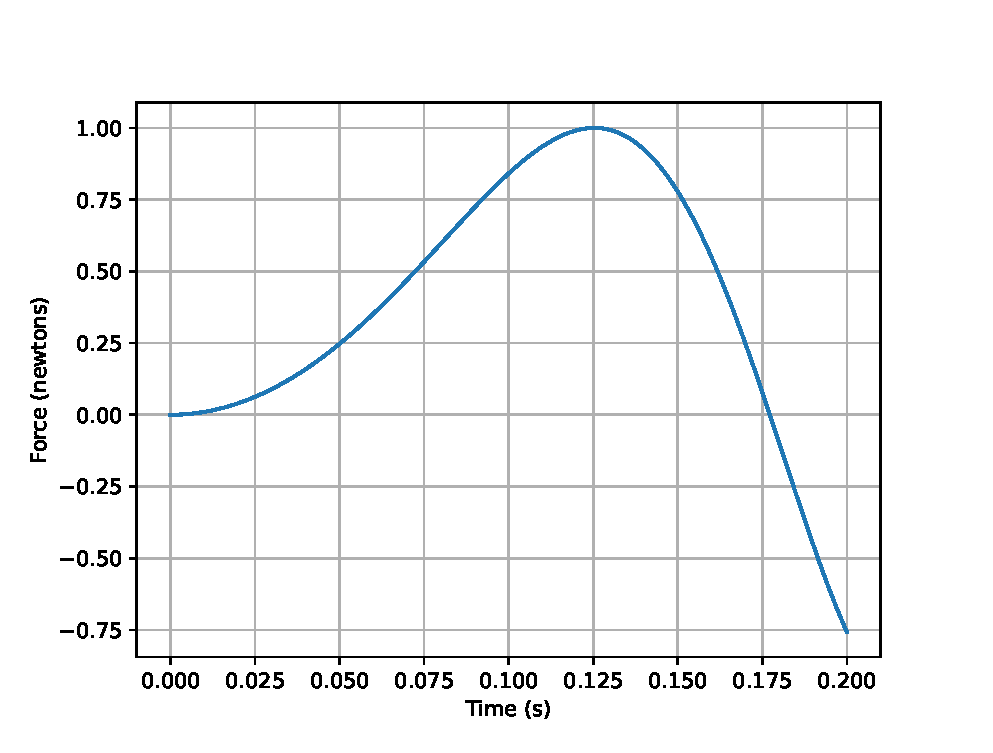
\includegraphics[width=0.8\linewidth]{imgs/q4_f_t.eps}
	\caption{Force over time}%
	\label{fig:14}
\end{figure}

\begin{figure}[H]
	\centering
	\captionsetup{justification=centering}
	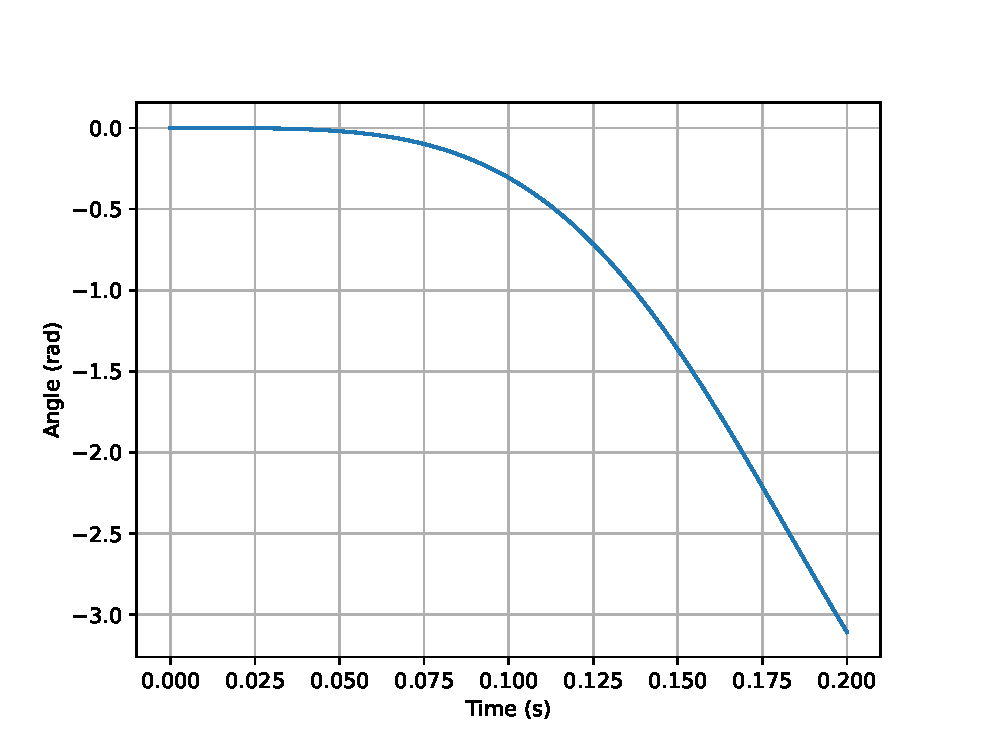
\includegraphics[width=0.8\linewidth]{imgs/q4_theta_t.eps}
	\caption{Angle over time}%
	\label{fig:14}
\end{figure}

\begin{figure}[H]
	\centering
	\captionsetup{justification=centering}
	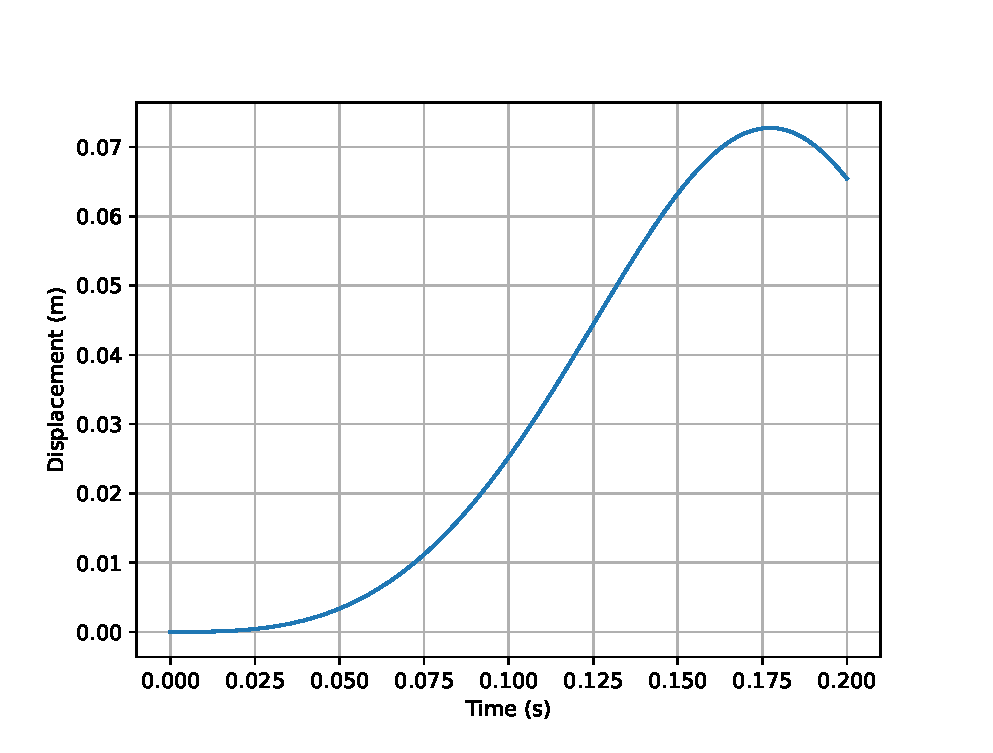
\includegraphics[width=0.8\linewidth]{imgs/q4_x_t.eps}
	\caption{Position over time}%
	\label{fig:14}
\end{figure}